% rubber: module xelatex
\documentclass[english,final,compress]{beamer}
%\usepackage[utf8]{inputenc}
\usepackage[T1]{fontenc}
\usepackage{fixltx2e}
\usepackage{graphicx}
\usepackage{longtable}
\usepackage{float}
\usepackage{wrapfig}
\usepackage{soul}
\usepackage{textcomp}
\usepackage{marvosym}
\usepackage{wasysym}
\usepackage{latexsym}
\usepackage{amssymb}
\usepackage{hyperref}
\tolerance=1000
\mode<beamer>{\usetheme{Bonn}}
\usepackage{fontspec}
\defaultfontfeatures{Mapping=tex-text}
\usepackage{xunicode}
\usepackage{xltxtra}
\setmainfont[Scale=0.86,Mapping=tex-text]{News Gothic MT}
\setsansfont[Scale=0.86,Mapping=tex-text]{News Gothic MT}
\setmonofont[Scale=0.86,Mapping=tex-text]{Andale Mono}
\usepackage{polyglossia}
\setdefaultlanguage{english}
\usepackage[EU1]{fontenc}
\usepackage{listings}
\usepackage{color}
\usepackage{csquotes}
\usepackage{mdwtab}
\usepackage{booktabs}
\usepackage{amsmath}
\usepackage{amssymb}
\usepackage{amstext}
\usepackage{amsthm}
\usepackage{listings}
\renewcommand\maketitle{\frame[plain]{\titlepage}\addtocounter{framenumber}{-1}}
\providecommand{\alert}[1]{\textbf{#1}}

\setbeamercolor{insult}{fg=black,bg=red!30}
\setbeamercolor{noinsult}{fg=black,bg=green!30}
\setbeamerfont*{myserif}{family=\rmfamily,size=\scriptsize}

\title{Tutorial Machine Learning in Python}
\author{Andreas M\"{u}ller, Hannes Schulz, Nenad Bire\v sev and Sven 
    Behnke\\[5mm]
\includegraphics[width=.2\linewidth]{style/Logo_UBo_h24_4c-crop}}
\date{ICANN 2012}
\begin{document}

\maketitle


\lstset{%
    basicstyle=\small\tt,
    keywordstyle=\color{beamer@bonnblue}\bfseries, % style for keywords
    numbers=none, % where to put the line-numbers
    numberstyle=\tiny, % the size of the fonts that are used for the line-numbers
    showspaces=false, % show spaces adding particular underscores
    showstringspaces=false, % underline spaces within strings
    showtabs=false, % show tabs within strings adding particular underscores
    tabsize=2, % sets default tabsize to 2 spaces
    captionpos=b, % sets the caption-position to bottom
    breaklines=true, % sets automatic line breaking
    breakatwhitespace=false, 
}
\newcommand\fenc{f_{\mathrm{enc}}}
\newcommand\fdec{f_{\mathrm{dec}}}
\newcommand\Wand{\ensuremath{W_{\mathbf{and}}}}
\newcommand\Wor{\ensuremath{W_{\mathbf{or}}}}
\newcommand{\w}[1]{\ensuremath{\mathbf{#1}}}
\newcommand\loss{\ell}

\frame[plain]{\frametitle{Outline}\tableofcontents\addtocounter{framenumber}{-1}}
\section{Introduction to Python}

%\begin{frame}
%    \frametitle{Machine Learning Overview}
%    \begin{itemize}
%        \item Intro: Sven
%        \item Python: Hannes
%        \item Before Lunch: Unsupervised Learning (Hannes)
%        \item After Lunch: Supervised Learning (Nenad LinReg, Andy LogReg/kNN)
%    \end{itemize}
%\end{frame}


\begin{frame}
    \frametitle{A Short Introduction to Python}
    \begin{itemize}
        \item Please log in, using:
            \begin{description}
                \item[Username] \alert{gkbionik}
                \item[Password] \alert{tut0rial} (with a zero instead of the 
                    ``o''!)
            \end{description}
    \end{itemize}
\end{frame}


\section{Unsupervised Learning}

\subsection{PCA}

%%% Local Variables: 
%%% mode: latex
%%% TeX-master: "presentation"
%%% End: 


\begin{frame}[fragile]
  \frametitle{Motivation: Exploring High-Dim Data}
  \begin{columns}
    \column{.5\linewidth}
    \begin{itemize}
    \item<1-> Let's say you do an experiment. 
    \item<1-> You vary very few variables, and measure many different outcome variables.
    \item<1-> In our example, we change one variable, but measure four.
    \item<2-> You'd suspect there is a \alert{simple low-dimensional
      structure} hidden in these four dimensions.
    \end{itemize}
    \column{.5\linewidth}
    varied:\\
    ~\footnotesize{\verb+Y=[0,1,2,1,1,0,2,0,...]+}

    observed:
\begin{verbatim}
X =
[[ 5.1  3.5  1.4  0.2]
 [ 4.9  3.   1.4  0.2]
 [ 4.7  3.2  1.3  0.2]
 [ 4.6  3.1  1.5  0.2]
 [ 5.   3.6  1.4  0.2]
 [ 5.4  3.9  1.7  0.4]
 [ 4.6  3.4  1.4  0.3]
 [ 5.   3.4  1.5  0.2]
 [ 4.4  2.9  1.4  0.2]
 ...
 [ 4.8  3.4  1.6  0.2]
 [ 4.8  3.   1.4  0.1]
 [ 4.3  3.   1.1  0.1]]
\end{verbatim}
  \end{columns}
\end{frame}

\begin{frame}[fragile]
  \frametitle{Plotting the Data}
  \begin{columns}
    \column{.5\linewidth}
    \begin{itemize}
    \item<1-> Looking at numbers is boring.
    \item<2-> 4 dimensions can be projected make 16 pairs
    \end{itemize}
    \column{.5\linewidth}
    \begin{onlyenv}<1>
\begin{lstlisting}
X =
[[ 5.1  3.5  1.4  0.2]
 [ 4.9  3.   1.4  0.2]
 [ 4.7  3.2  1.3  0.2]
 [ 4.6  3.1  1.5  0.2]
 [ 5.   3.6  1.4  0.2]
 [ 5.4  3.9  1.7  0.4]
 [ 4.6  3.4  1.4  0.3]
 [ 5.   3.4  1.5  0.2]
 [ 4.4  2.9  1.4  0.2]
 ...
 [ 4.8  3.4  1.6  0.2]
 [ 4.8  3.   1.4  0.1]
 [ 4.3  3.   1.1  0.1]]
\end{lstlisting}
    \end{onlyenv}
    \includegraphics<2>[width=\linewidth]{pca-pics/iris-all}
  \end{columns}
\end{frame}

\begin{frame}[plain]
  \begin{center}
   
    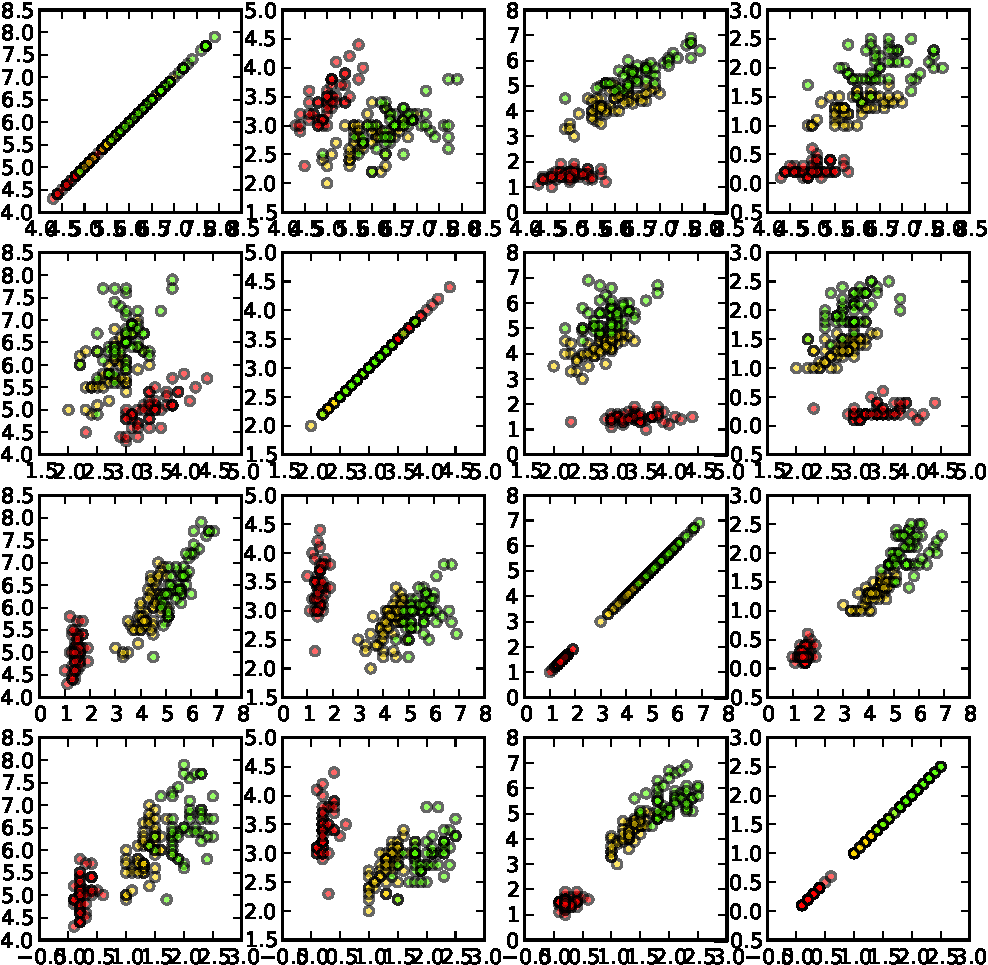
\includegraphics[height=.99\textheight]{pca-pics/iris-all}

  \end{center}
\end{frame}

\begin{frame}
  \frametitle{Plotting the Data}
  \begin{columns}
    \column{.5\linewidth}

    \begin{enumerate}
    \item<1-> Which one of those projections is \alert{good}?
    \item<2-> Are there others, possibly \alert{better} projections?
    \item<3-> \alert{Which variables} are involved in the best
      projections?
    \end{enumerate}
    \column{.5\linewidth}
    \includegraphics<1->[width=\linewidth]{pca-pics/iris-all}
  \end{columns}
\end{frame}

\begin{frame}[fragile]
  \frametitle{Principal Component Analysis}
  \begin{itemize}
  \item PCA projects to axis with greatest \alert{variance}
  \item Often provides good \alert{first insight} into dataset
  \end{itemize}

  \begin{columns}
    \column{.5\linewidth}
    \begin{align*}
        P &\leftarrow \mathrm{PCA}(X-m, 2)\\
        X_{\mathrm{PCA}} & \leftarrow P (X-m)
    \end{align*}
    \column{.5\linewidth}
    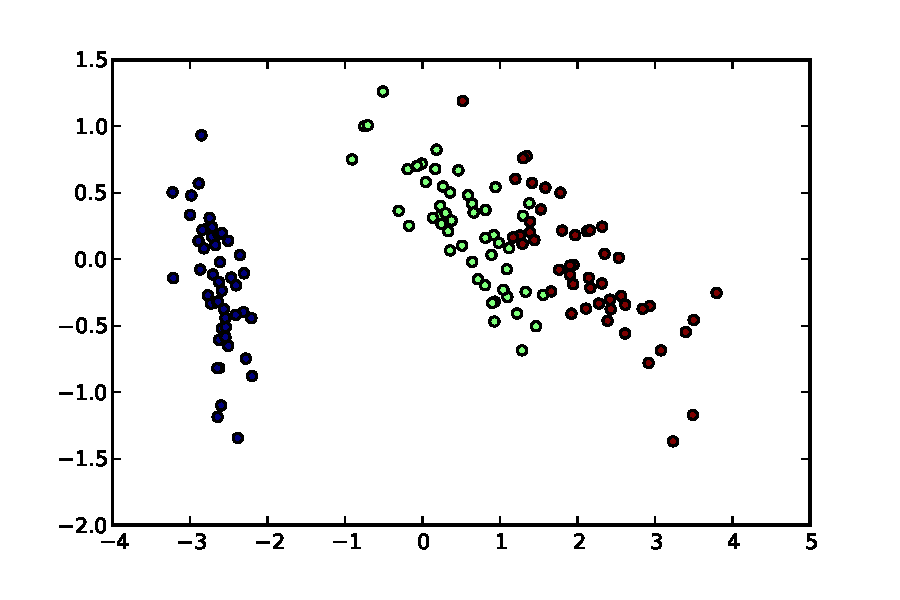
\includegraphics[width=.99\linewidth]{pca-pics/iris-2d}
  \end{columns}

  \pause
  \begin{itemize}
  \item Important variables: Take a look at the projection matrix $P$:
  \end{itemize}

  \begin{lstlisting}[escapechar=!]
    P = [[ 0.36 -0.08 !\alert<3>{0.85}! 0.35]
         [!\alert<4>{-0.65}! !\alert<4>{-0.72}  0.17  0.07]]
  \end{lstlisting}
\end{frame}

\begin{frame}[fragile]
  \frametitle{Noise Reduction}
  \begin{columns}
      \begin{column}{.7\linewidth}
          \begin{itemize}
              \item Most of the data explained by first axes
              \item (almost) constant axes thrown away
              \item Projecting back to input-space reduces noise
          \end{itemize}
      \end{column}
      \begin{column}{.3\linewidth}
          \begin{align*}
              X_{\mathrm{clean}} \rightarrow X_{\mathrm{PCA}} P + m 
          \end{align*}
      \end{column}
  \end{columns}
  \begin{center}
    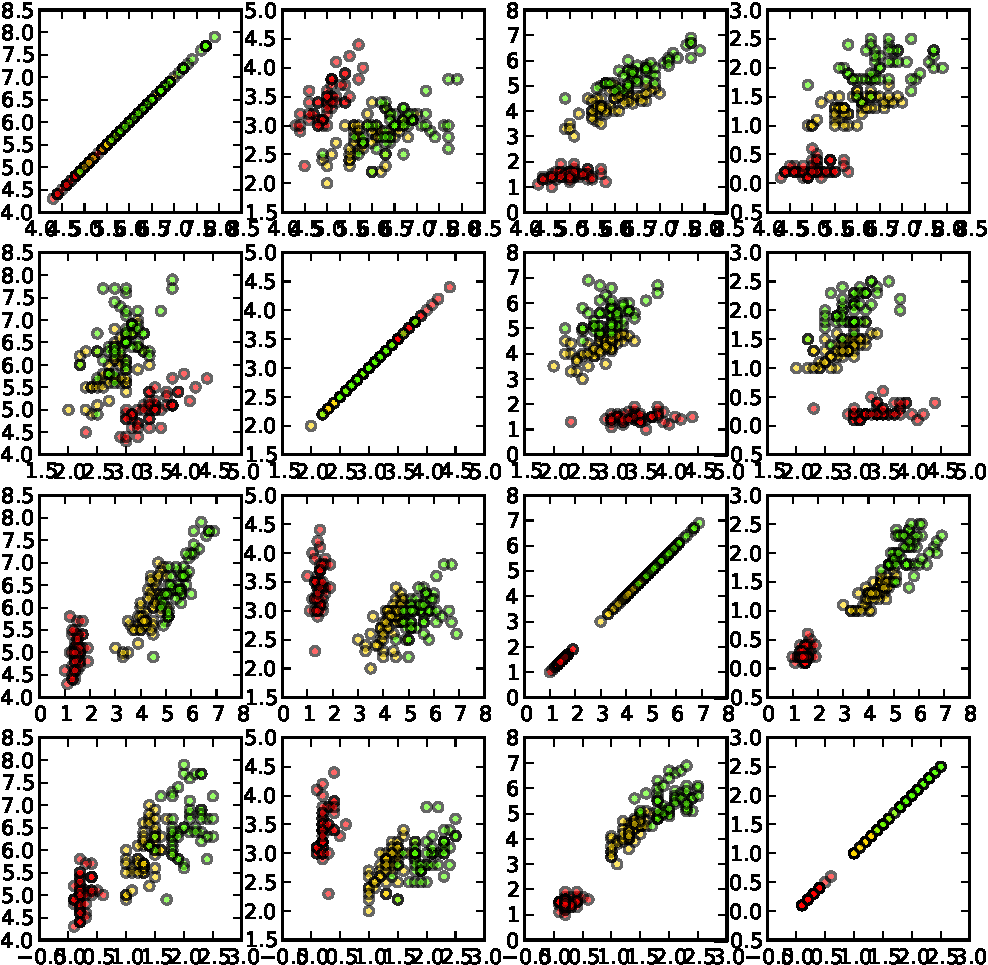
\includegraphics[width=.47\linewidth]{pca-pics/iris-all}\hfill%
    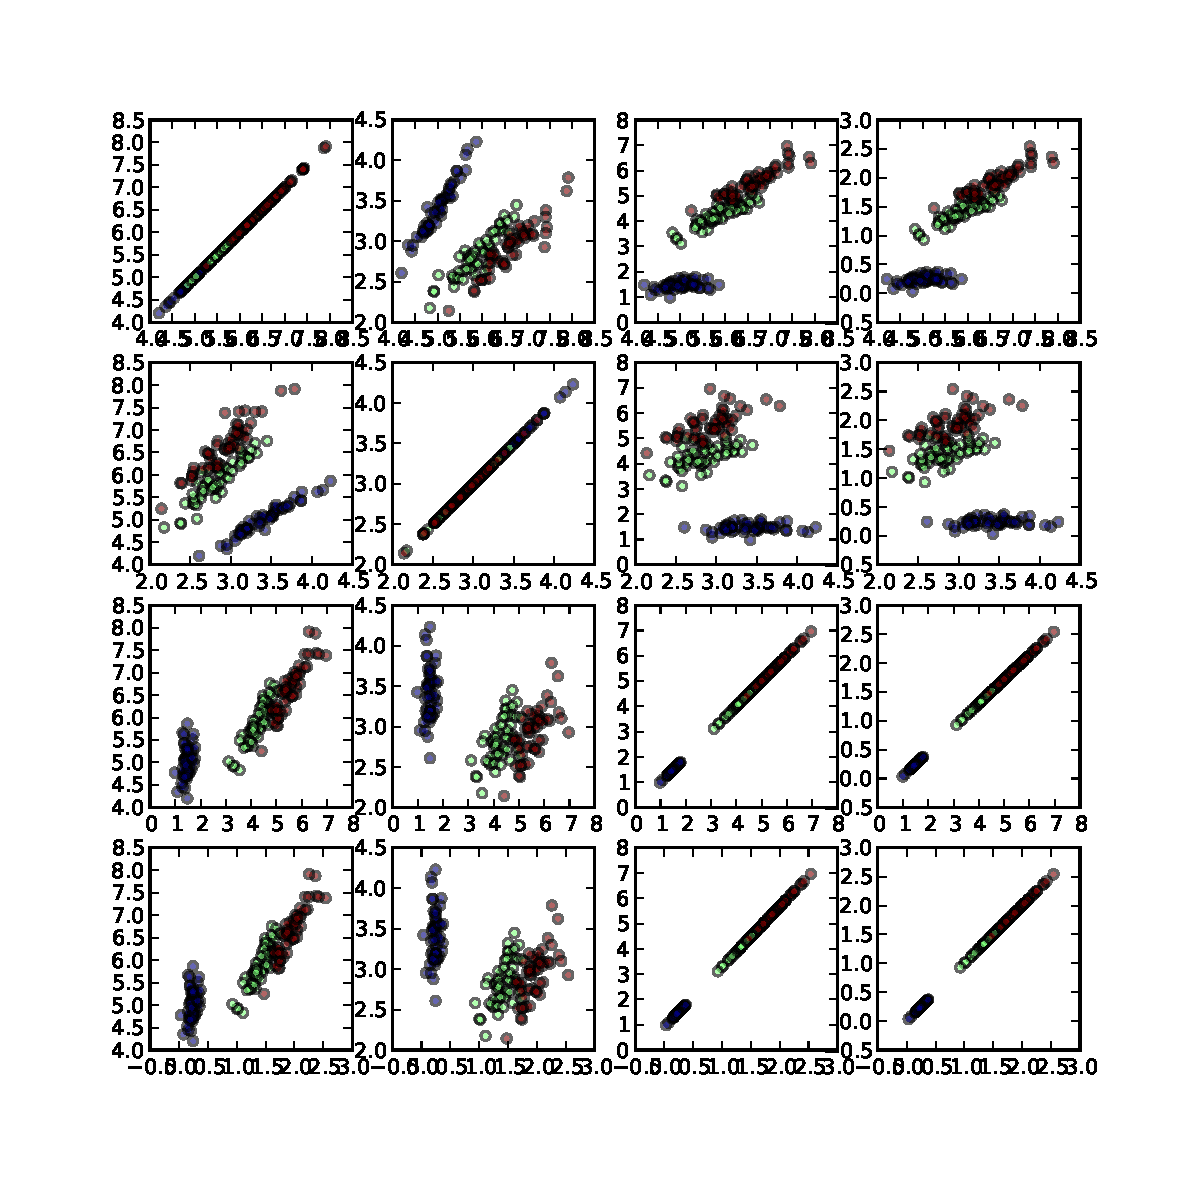
\includegraphics[width=.47\linewidth]{pca-pics/iris-bt}
  \end{center}
\end{frame}




\subsection{k-Means}

\begin{frame}
    \frametitle{k-Means}

    
\end{frame}

\begin{frame}
    \frametitle{k-Means -- Interactive}
    \begin{itemize}
        \item  find blobs on artificial data
        \item  color discretization in an image (TODO: bio images (--> Kristian and Baukhage?))
        \item  visualize cluster centers in "interesting data" (TODO: data??)
    \end{itemize}
\end{frame}



\section{Supervised Learning}


\begin{frame}
    \frametitle{Supervised Learning -- General}
    \begin{itemize}
	\item Task: Learn the function $ y = f(X) $ which predicts the output $y$ for the given input $X$, knowing the desired output
        \item Each example in data is a tuple of the input and desired output (target)
    \end{itemize}
\end{frame}


\begin{frame}
    \frametitle{Example: Supervised Learning}
    \begin{itemize}
       \item Input Data: 40 examples of persons (age, height, smoker, nationality). 
	\item Targets: Weight of the person (desired output)
	\item Goal: Learn a function which predicts the weight for the new person
		knowing the age, height, smoker, nationality of person.

    \end{itemize}
\end{frame}

\begin{frame}
    \frametitle{Training / Test data}
    \begin{itemize}
	\item Learning is done on the training data, for which we know the input and targets
	\item To test if the model learned to predict the output, we use test data. 		
    \end{itemize}
\end{frame}

\subsection{Linear Regression}

\begin{frame}
    \frametitle{Linear Regression}
    \begin{columns}
        \column{.5\linewidth}
            \begin{itemize}
                \item Task: for the given input $x$ predict the real value output $y = f(x)$ 
                \item Fit a hyperplane to data 
                \item Linear  function: simple, easy to understand.
            \end{itemize}
        \column{.5\linewidth}
            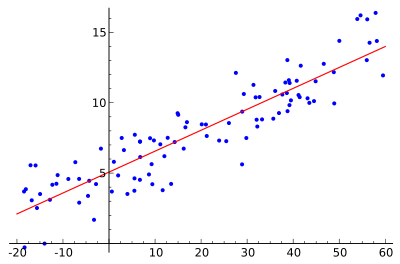
\includegraphics[width=1\linewidth]{linreg-pics/lg2}\\

    \end{columns}
\end{frame}


\begin{frame}
    \frametitle{Example: Okuns Law Quarterly Differences}
    \begin{columns}
        \column{.5\linewidth}
            \begin{itemize}
                \item Data: quarterly change in unemployment rate 
                \item Predict: quarterly change in GDP
            \end{itemize}
        \column{.5\linewidth}
            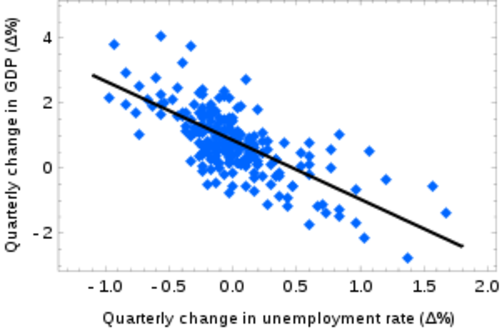
\includegraphics[width=1\linewidth]{linreg-pics/lg}\\

    \end{columns}
\end{frame}


\begin{frame}
    \frametitle{Mathematical Formulation I}
            \begin{itemize}
                \item Linear function: $y = \sum_{i=1}^{N} w_i x_i + b$
                \item $x_i$ - input    
                \item $w_i$ - weights 
                \item $b$ - bias
                \item $y$ - output
            \end{itemize}
\end{frame}


\begin{frame}
    \frametitle{Example for Hyperplane}
    \begin{columns}
        \column{.5\linewidth}
            \begin{itemize}
                \item $y =  w_1 x + b$
                \item How do we find coefficients $w_i$ ? 
            \end{itemize}
        \column{.5\linewidth}
            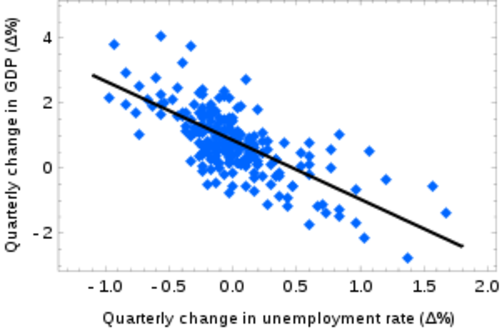
\includegraphics[width=1\linewidth]{linreg-pics/lg}\\

    \end{columns}
\end{frame}





\begin{frame}
    \frametitle{Mathematical Formulation II}
    \begin{columns}
        \column{.5\linewidth}
            \begin{itemize}
                \item Minime the distance between each data point and the line
                \item $ E = \sum_{i=0}^{N}(y_i - (w x_i + b))$
                \item Linear regression finds the weights for which the error $E$ is minimal
            \end{itemize}
        \column{.5\linewidth}
            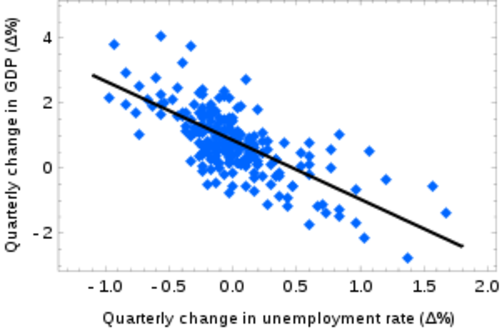
\includegraphics[width=1\linewidth]{linreg-pics/lg}\\
    \end{columns}
\end{frame}


\begin{frame}
    \frametitle{Example: 2D Data}
    \begin{columns}
        \column{.5\linewidth}
            \begin{itemize}
                \item What if our input data has 2-dim?
                \item We can see some linear relationship in the data
            \end{itemize}
        \column{.5\linewidth}
            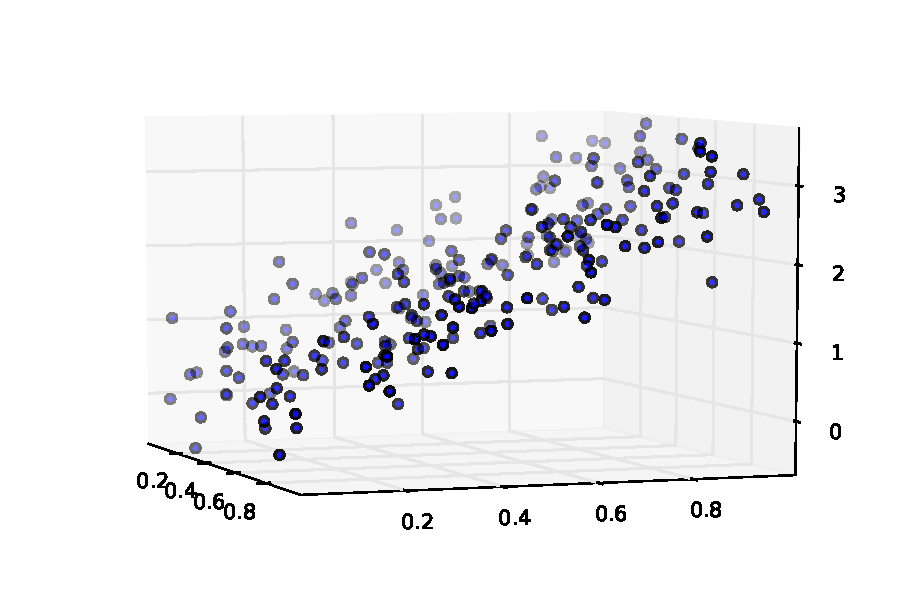
\includegraphics[width=1\linewidth]{linreg-pics/only_data}\\

    \end{columns}
\end{frame}



\begin{frame}
    \frametitle{Example: 2D Data}
    \begin{columns}
        \column{.5\linewidth}
            \begin{itemize}
                \item This time, we are fitting the plane
                \item $y =  w_2 x_2 + w_1 x_1 + b$

            \end{itemize}
        \column{.5\linewidth}
            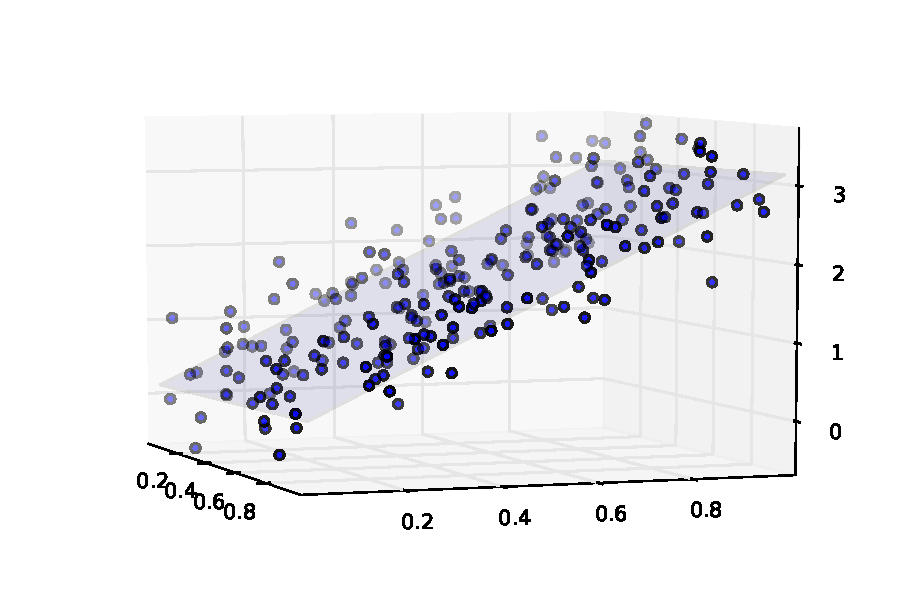
\includegraphics[width=1\linewidth]{linreg-pics/with_plane}\\
            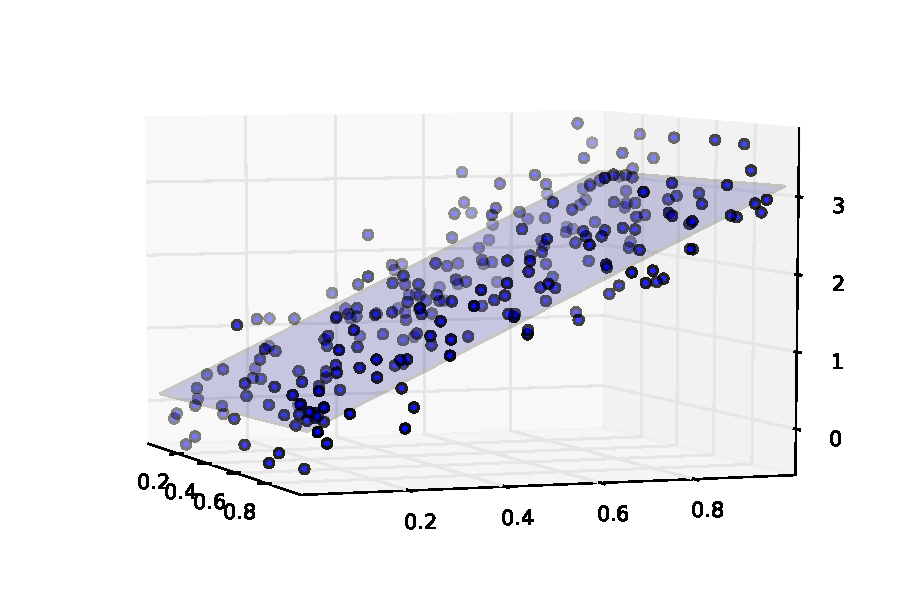
\includegraphics[width=1\linewidth]{linreg-pics/lin_reg_plane}\\

    \end{columns}
\end{frame}


\begin{frame}
    \frametitle{Linear Regression -- Interactive}
    \begin{itemize}
        \item Open Notebook titled 3a - Linear regression 1D.
    \end{itemize}
\end{frame}



\subsection{Classification}
\begin{frame}
    \frametitle{Classification}
    \begin{itemize}
        \item Predict to which class a data point belongs.
        \item Training data are pairs $\left( (x_0, y_0), \cdots, (x_N, y_N)
                \right), x_i \in \mathbb{R}^n, y_i \in \{0, \cdots, k\}$
        \item Classical example: Spam / Ham.
        \item All classes known beforehand.
        \item Other examples: Digit recognition, cancer benign/malignant, \ldots
    \end{itemize}
\end{frame}

\subsection{Logistic Regression}

\begin{frame}
    \frametitle{Logistic Regression}
    \begin{columns}
        \column{.5\linewidth}
            \begin{itemize}
                \item Misnamed: Classification, not regression.
                \item Linear decision function: simple, easy to understand.
            \end{itemize}
        \column{.5\linewidth}
            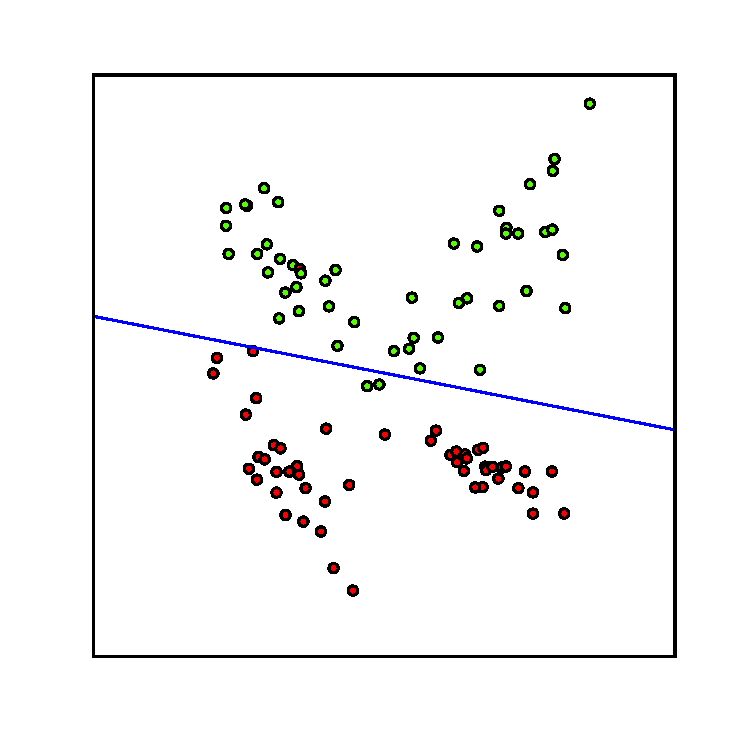
\includegraphics[width=1\linewidth]{logreg-pics/synthetic_line}\\

    \end{columns}
\end{frame}

\begin{frame}
    \frametitle{Example: Wisconsin Breast Cancer}
    \begin{columns}
        \column{.5\linewidth}
            \begin{itemize}
                \item Classify breast cancer samples in malign or benign.
                \item 700 Samples with 10 measurements each.
                \item We take only 3 measurements:
                    \begin{itemize}
                        \item Uniformity of Cell Size
                        \item Uniformity of Cell Shape
                        \item Single Epithelial Cell Size
                    \end{itemize}
                \item Training on 525, test on 175
                \item 97.1\% Accuracy
            \end{itemize}
        \column{.5\linewidth}
            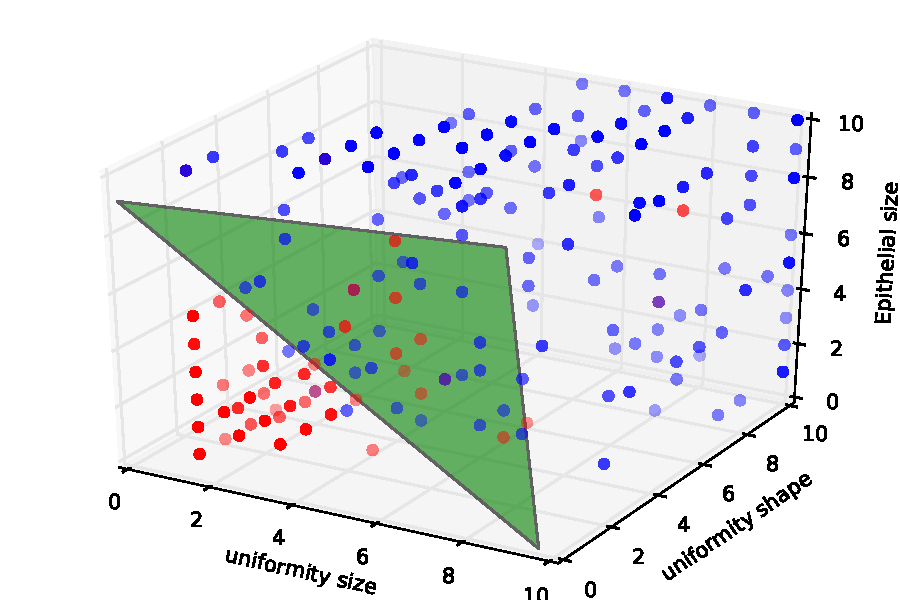
\includegraphics[width=1\linewidth]{logreg-pics/wisconsin_surface}
    \end{columns}

\end{frame}

\begin{frame}
    \frametitle{Mathematical Formulation I}
    \begin{columns}
        \column{.5\linewidth}
        \begin{itemize}
            \item For two classes $-1, +1$.
            \item Decision boundary given by hyperplane.
            \item Hyperplane defined by normal vector and offset:
                \begin{gather*}
                    y = \text{sign}(\left<w, x\right> + b)\\
                    w \in \mathbb{R}^n, b \in \mathbb{R}
                \end{gather*}
        \end{itemize}
        \column{.5\linewidth}
            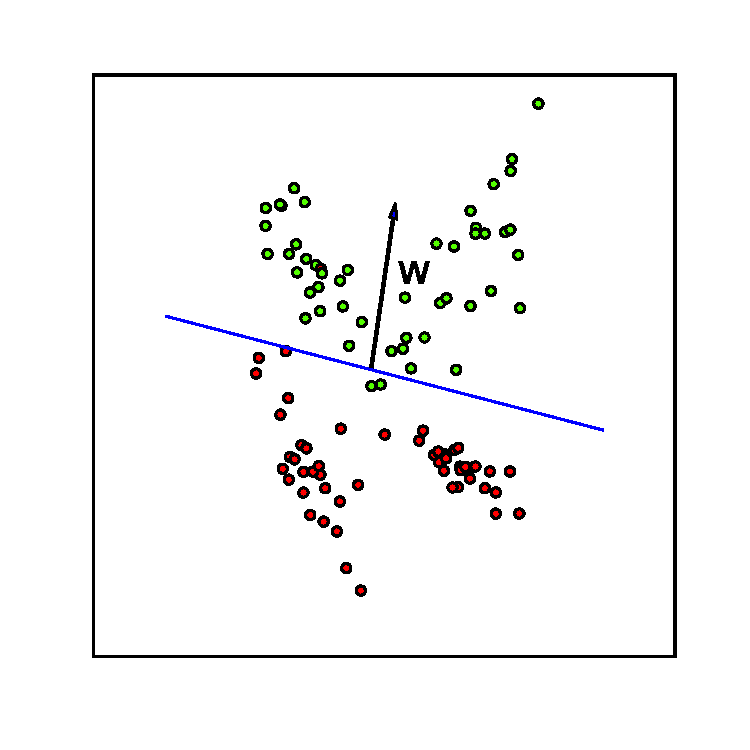
\includegraphics[width=1\linewidth]{logreg-pics/synthetic_line_w}\\

    \end{columns}
\end{frame}

\begin{frame}
    \frametitle{Mathematical Formulation II}
    \begin{columns}[T]
        \column{.5\linewidth}
            \begin{itemize}
                \item Relation to regression:
                    \begin{align*}
                        p(y=+1\,|\, x) = \text{logistic}(\left<w, x\right> + b)
                    \end{align*}
                \item As probabilities are between $0$ and $1$, the logistic function
                    squashes the regression result:
                    \begin{align*}
                         p(y=+1 \,|\, x) > 0.5 \Leftrightarrow \left <w, x \right> + b > 0
                     \end{align*}
            \end{itemize}
        \column{.4\linewidth}
            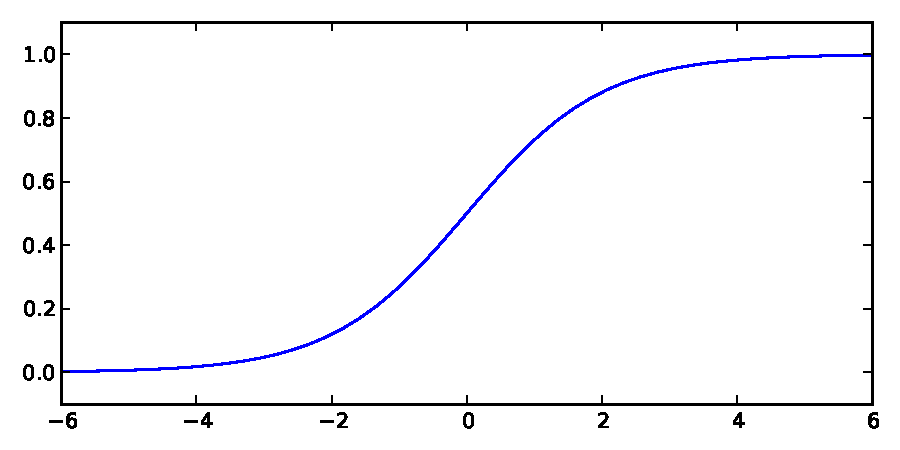
\includegraphics[width=.8\linewidth]{logreg-pics/logistic_sigmoid}\\
    \end{columns}
    \begin{itemize}
        \item Need to solve:
            \begin{align*}
                \max_w \sum_{i=0}^n \log(p(Y=y_i | x_i))
            \end{align*}
    \end{itemize}
\end{frame}


\begin{frame}
    \frametitle{Example: Classifying Insults I}
    \begin{columns}
        \column{.5\linewidth}
        \begin{itemize}
            \item Dataset: Forum posts / comments on social issues.
            \item Two classes: Insulting towards other posters / not insults.
            \item Training set: 4000 comments, test set: 2500 comments
            \item Features: Extract dictionary of all occuring words, count occurence per comment.
            \item Very high dimensional: 16.500
            \end{itemize}
        \column{.5\linewidth}
            \begin{beamercolorbox}[sep=1em,wd=5cm]{insult}
                \usebeamerfont{myserif}Either you are fake or extremely stupid\dots maybe both\dots\\
            \end{beamercolorbox}
            \vspace{1em}

            \begin{beamercolorbox}[sep=1em,wd=5cm]{noinsult}
                \usebeamerfont{myserif}i really don't understand your point. It seems that you are
                mixing apples and oranges.\\
            \end{beamercolorbox}
            \vspace{1em}

            \begin{beamercolorbox}[sep=1em,wd=5cm]{insult}
                \usebeamerfont{myserif}To engage in an intelligent debate with
                you is like debating to a retarded person.  It's useless.  It
                looks like you're bent on disregarding the efforts of the
                government.
            \end{beamercolorbox}
            \vspace{1em}

            \begin{beamercolorbox}[sep=1em,wd=5cm]{noinsult}
                \usebeamerfont{myserif}@jdstorm dont wish him injury but it happened on its OWN and i
                DOUBT he's injured, he looked embarrassed to me\\
            \end{beamercolorbox}
    \end{columns}
\end{frame}


\begin{frame}[t]
    \frametitle{Example: Classifying Insults II}
    \begin{columns}[t]
        \column{.4\linewidth}
            \begin{beamercolorbox}[sep=1em,wd=5cm]{insult}
                \usebeamerfont{myserif}Either you are fake or extremely stupid\dots maybe both\dots\\
            \end{beamercolorbox}
        \column{.4\linewidth}
            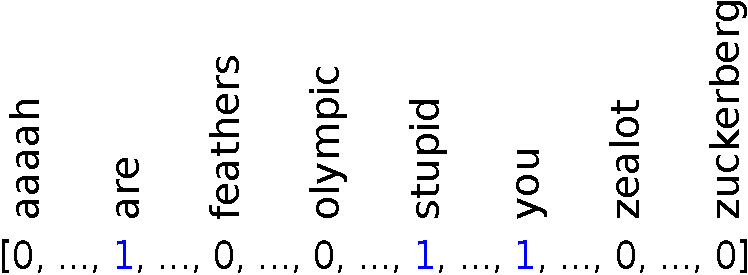
\includegraphics[width=.9\linewidth]{logreg-pics/bag_of_words-crop}\\
            
    \end{columns}
    \vspace{3mm}
    \begin{onlyenv}<2->
        Accuracy with logistic regression: 84.5\%\\
    \end{onlyenv}
    \vspace{3mm}
    \begin{onlyenv}<3>
        The largest coefficients (sign given by color):
        \begin{center}
            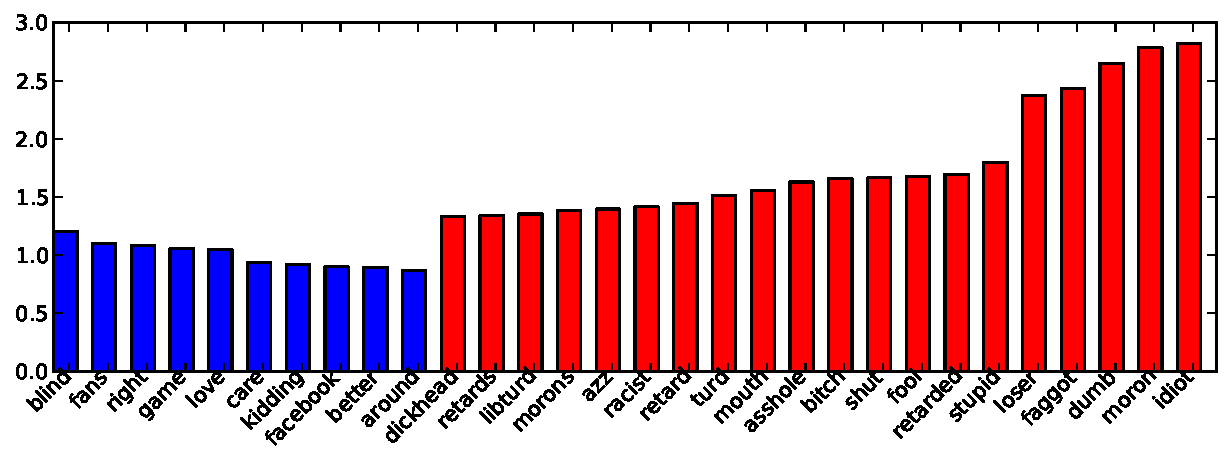
\includegraphics[width=.9\linewidth]{logreg-pics/bow_coef}
        \end{center}
    \end{onlyenv}
\end{frame}

\begin{frame}
  \frametitle{Interactive Part}
  \begin{itemize}
      \item Open Notebook titled ``4 - Logistic Regression''.
      \item If your screen is locked, the password is tut0rial.
  \end{itemize}
\end{frame}


\subsection{$k$ Nearest Neighbors}

\begin{frame}
    \frametitle{$k$ Nearest Neighbors}
    \begin{itemize}
        \item Classification: same setup as logistic regression.
        \item Very simple but powerful idea: Do as your neighbors does.
        \item For a new point $x$ look at the nearest (or the two nearest or three nearest, \ldots)
            point in the training data for a label.
        \item Usually: Euclidean distance in $\mathbb{R}^n$
    \end{itemize}
\end{frame}

\begin{frame}
    \frametitle{Simple algorithm}
    \begin{itemize}
        \item Pick a $k$, for example $k=3$.
        \item Want to classify new example $x$.
        \item Compute $d_i = d(x_i, x)$, i.e.\, $d(x_i, x) = ||x_i - x||$
        \item Sort $d_i$, take $k$ smallest: $d_{i_0}, d_{i_1}, d_{i_2}$.
        \item Assign $y$ that appears most often among $y_{i_0}, y_{i_1}, y_{i_2}$
    \end{itemize}
\end{frame}

\begin{frame}
    \frametitle{Illustration}
    \begin{center}
    \includegraphics<1>[width=.6\linewidth]{knn-pics/two_moons}
    \includegraphics<2>[width=.6\linewidth]{knn-pics/two_moons_k=5}
    \end{center}
\end{frame}

\begin{frame}
    \frametitle{Picking $k$}
    \begin{itemize}
        \item General problem called model selection.
        %\item Model selection is necessary for nearly all algorithms.
        \item For training data, $k=1$ gives perfect prediction -- but not for new data!
        %\item Larger $k$ leads to smoother boundaries and worse performance on the training set,
            %but better on the test set.
    \end{itemize}
    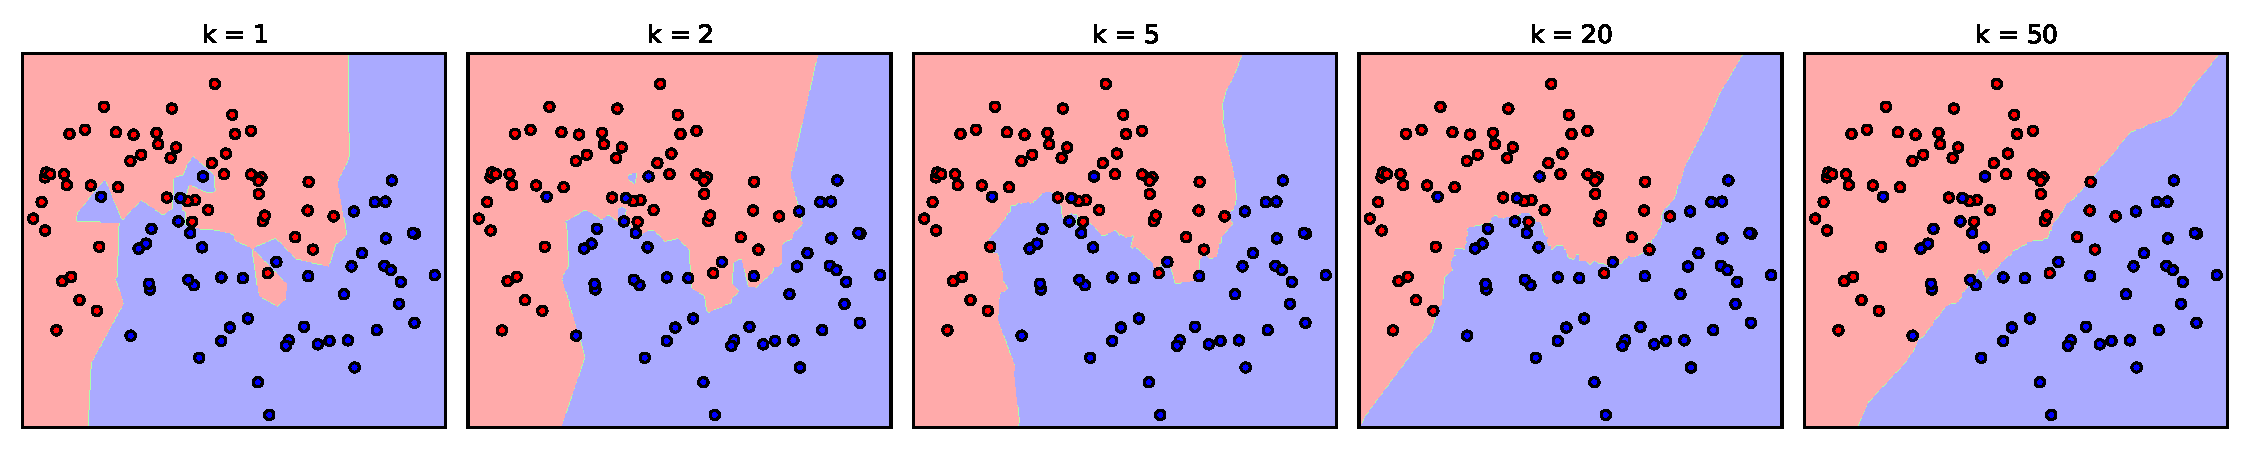
\includegraphics[width=.98\linewidth]{knn-pics/two_moons_varying_k}
\end{frame}


\begin{frame}[t]
    \frametitle{Picking $k$ (in practice)}
    \begin{itemize}
        \item We can not choose $k$ on the training set.
        \item We can not choose $k$ on the set we evaluate our algorithm on (or
            for that we need predictions).
    \end{itemize}
    \center
        \begin{onlyenv}<2>
            
\includegraphics[width=.7\linewidth]{knn-pics/train_test_bars-crop}\\
        \end{onlyenv}
        \begin{onlyenv}<3->
            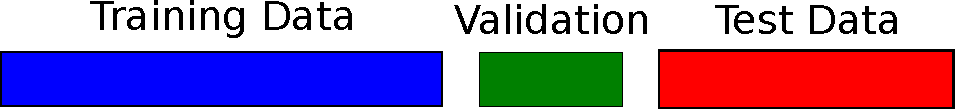
\includegraphics[width=.7\linewidth]{knn-pics/train_val_test_bars-crop}\\
        \end{onlyenv}

    \includegraphics<4>[width=.7\linewidth]{knn-pics/two_moons_cross_validation_1}
    \includegraphics<5>[width=.7\linewidth]{knn-pics/two_moons_cross_validation_2}
    \includegraphics<6>[width=.7\linewidth]{knn-pics/two_moons_cross_validation_3}

\end{frame}

%\begin{frame}
    %\frametitle{$k$ Nearest Neighbor -- Interactive}
    %\begin{itemize}
        %\item  start with blobs from k-means
        %\item  Iris dataset
        %\item  Measure prediction error
        %\item  Maybe: Complexity curve visualization (needs a loop)
    %\end{itemize}
%\end{frame}


\end{document}
